\chapter{Metodología}
El desarrollo de este trabajo se ha dividido en tres partes bien diferenciadas: los dos generadores,
tanto de perfiles energéticos como de consumo, y el gestor inteligente de carga de EVs.\\


Para la creación de dichos perfiles de consumo, se han empleado técnicas de IA Generativa, con el 
objetivo de obtener una gran variedad de perfiles de consumo, partiendo del dataset ya obtenido, 
con limitado número de muestras. Estos perfiles se han generado de forma que representen 
adecuadamente la variabilidad de la demanda energética para la carga de un EV, teniendo en cuenta
las restricciones, requisitos y hábitos del usuario. En segundo lugar, la generación de consumos 
energéticos se ha llevado a cabo usando LPG.\\

La implementación del código relevante para el proyecto se ha realizado en Python, utilizando
una serie de librerías y herramientas a disposición de estas tareas. Para la resolución del 
problema de optimización clásico, se ha hecho uso de la librería \textit{PyOmo}, con 
\textit{GurobiPy} como solver. Para el desarrollo de todo lo relacionado con aprendizaje profundo, 
se han empleado las librerías de \textit{Torch}.\\

\begin{figure}[ht]
    \centering
    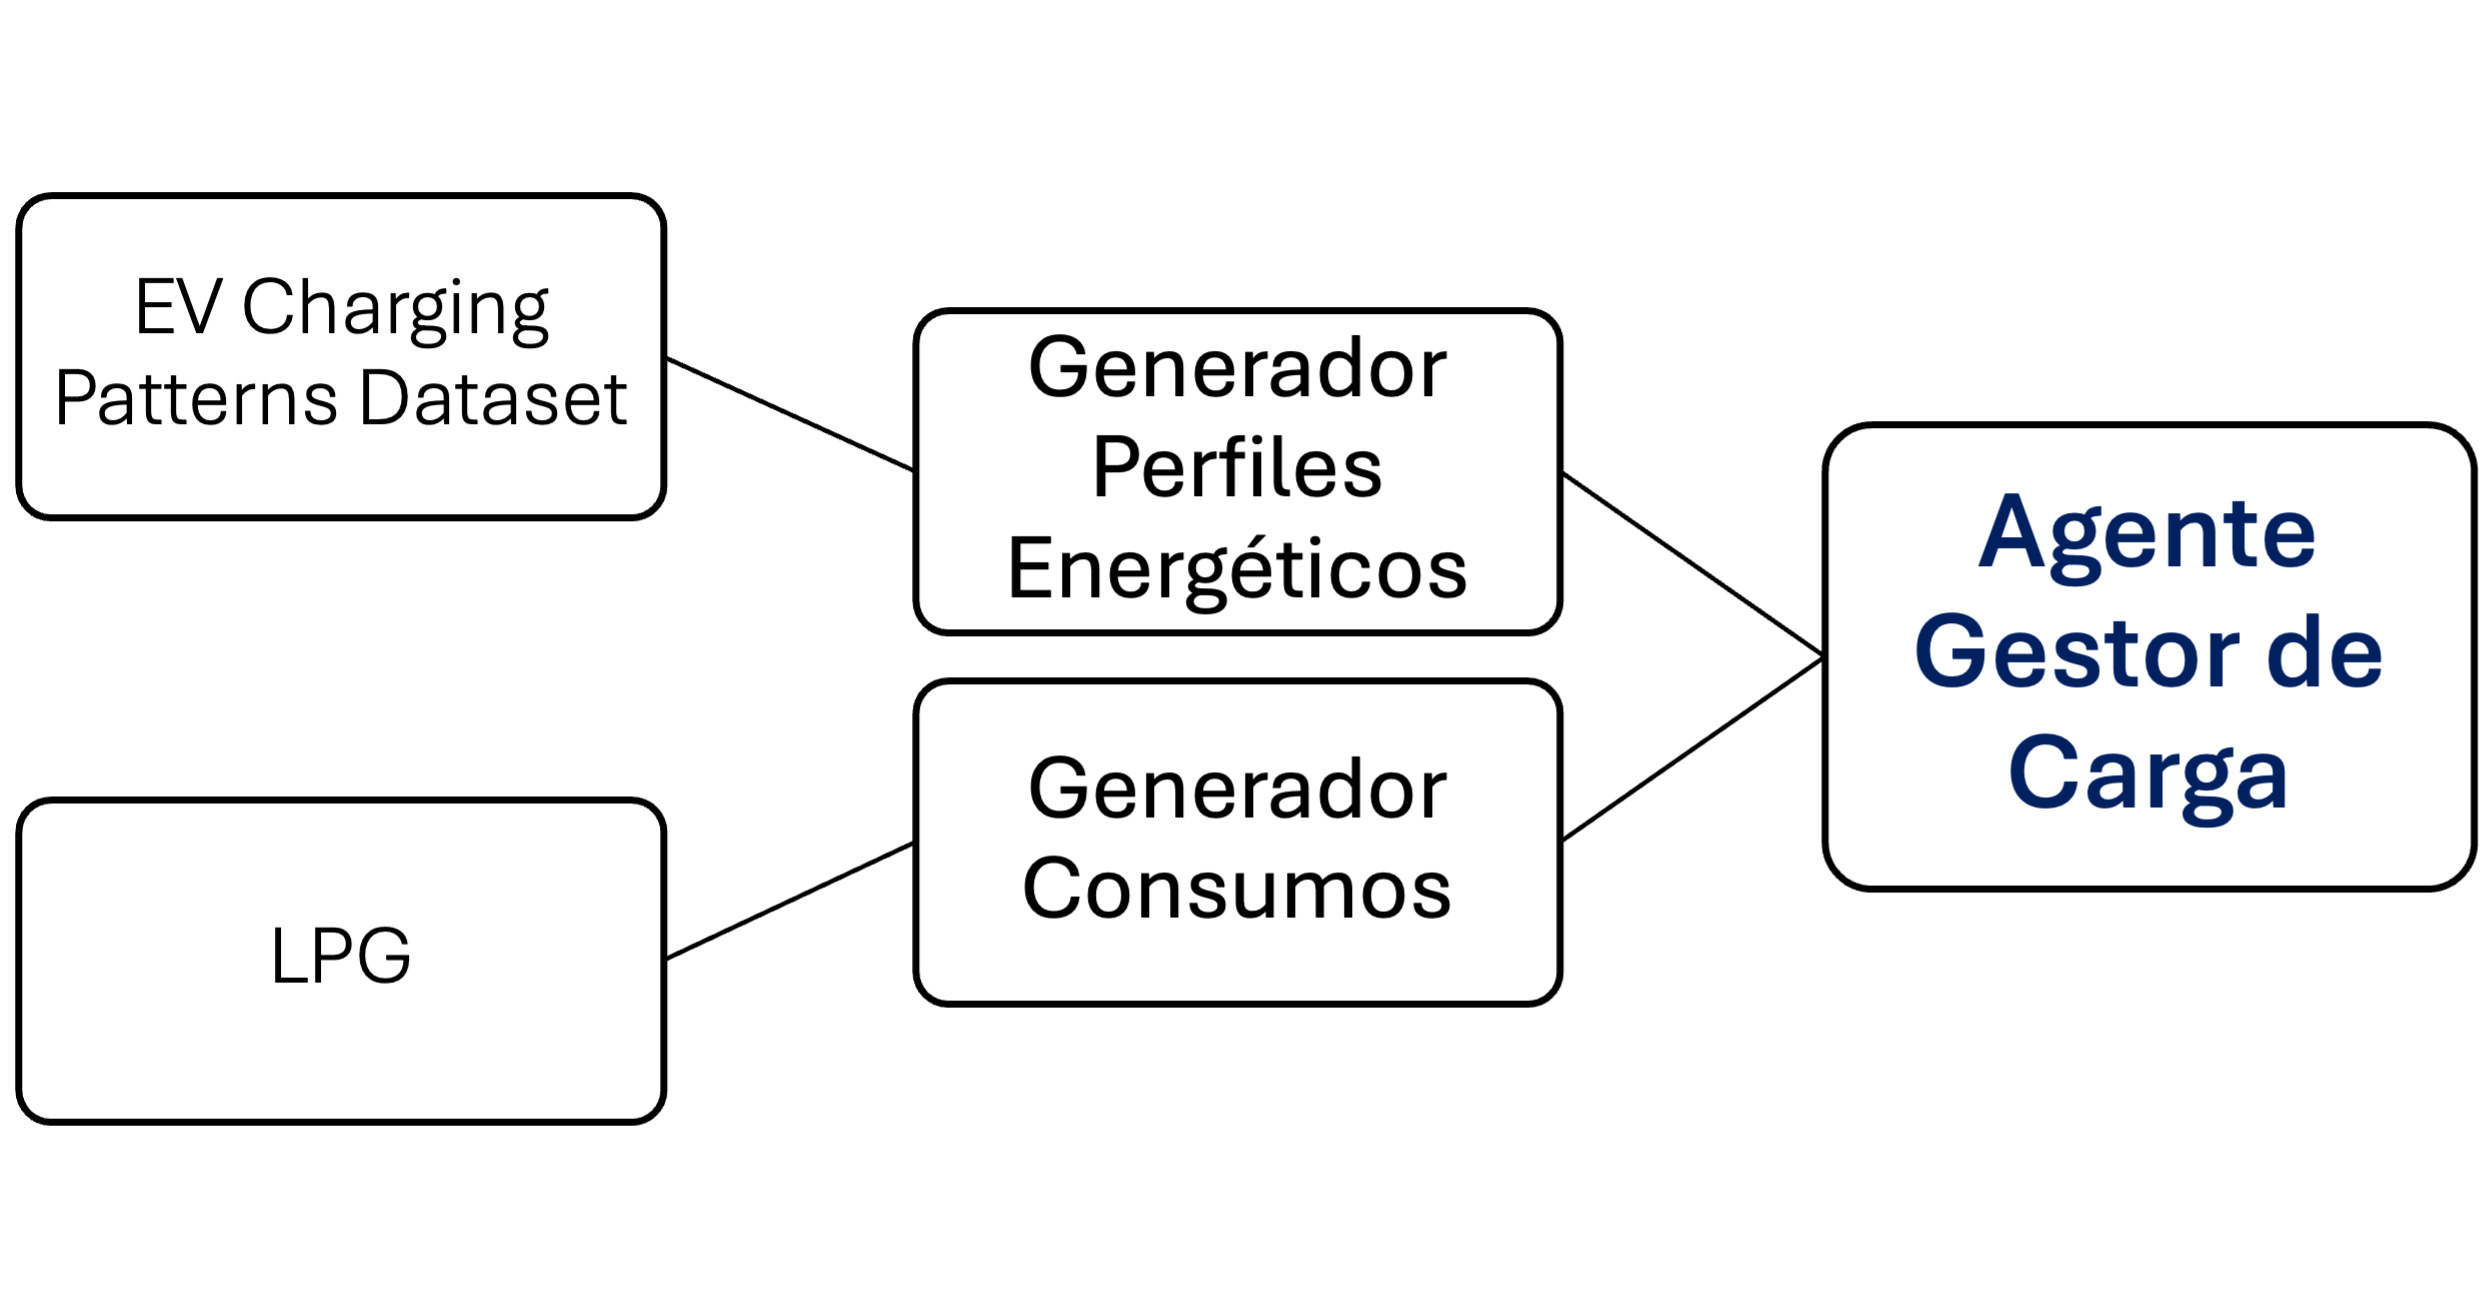
\includegraphics[width=1\textwidth]{images/metodologia.png}
    \caption{Metodología utilizada en el trabajo. Fuente: Elaboración propia.}
    \label{fig:metodologia}
\end{figure}

La metodología utilizada en este trabajo se ha diseñado para abordar de manera sistemática y 
efectiva los objetivos planteados. La Figura~\ref{fig:metodologia} ilustra las etapas clave del 
proceso, que incluyen la recopilación de datos, el análisis de la información, el desarrollo de 
modelos predictivos y la implementación de estrategias de gestión de la demanda.\\